\documentclass[conference]{IEEEtran}
\IEEEoverridecommandlockouts
\usepackage{amsmath,amssymb,amsfonts}
\usepackage{graphicx}
\usepackage{textcomp}
\usepackage{xcolor}
\usepackage{caption}
\usepackage{subcaption}

%added by Ye
\usepackage{fontspec}
%for typing Myanmar text, you can also used with Myanmar3 font
\newfontfamily {\padauktext}[Script=Myanmar]{Padauk}
%for double quote
\newcommand{\quotes}[1]{``#1''}
\renewcommand{\baselinestretch}{0.75}

\def\BibTeX{{\rm B\kern-.05em{\sc i\kern-.025em b}\kern-.08em
    T\kern-.1667em\lower.7ex\hbox{E}\kern-.125emX}}
\begin{document}

\title{Three Most Favorite Books that I've ever read\\(Recommeneded Books)}

\author{\IEEEauthorblockN{1\textsuperscript{st} Haymar Phyoe}
\IEEEauthorblockA{\textit{@ Software Lab, UT-YCC} \\
Pyin-Oo-Lwin \\
haymarphyoe777@gmail.com}
}

\maketitle

\begin{abstract}
\setlength{\parskip}{6pt}
{\padauktext
ယနေ့ လူငယ်၊ နောင်ဝယ် လူကြီး ဟု ဆိုကြသကဲ့သို့ ယနေ့  လူငယ်များသည် အနာဂတ်၏ ခေါင်းဆောင် များ ဖြစ်ကြသည်။ နိုင်ငံတော်၏ အနာဂတ်အားမာန် များဖြစ်သည့် လူငယ်များကို ငယ်ရွယ် နုနယ် သော ကလေးအရွယ် ကတည်းကပင် ကောင်းမွန်သည့် စိတ်ဓာတ်၊ စည်းကမ်း၊ ပညာများနှင့် ပြည့်စုံရန် ပြုစုပျိုးထောင် ရာ၌ စာပေသည်လည်း အရေးကြီးသည့် ကဏ္ဍတစ်ခု အနေဖြင့် ပါဝင်နေပါသည်။ စာပေသည် လူငယ်များ အတုယူ ရမည့် စိတ်နေ သဘောထားများ၊ ကြိုးစားချင်သော၊ သင်ယူလို သော၊ တီထွင်ဆန်းသစ်လိုသော အတွေးအခေါ်များ၊ မျိုးချစ် စိတ်ဓာတ် ရှင်သန်ထက်မြက်ရေး အစရှိသည့် စိတ်ဓာတ် ကောင်းတို့ကို ဖန်တီးပေးနိုင်သည်။ ရသစာပေ သည် လူငယ်များအား လူ့အကြောင်းနှင့် လူ့လောက အကြောင်းအရာများကို စွဲမြဲစေခဲ့သည်။ သုတစာပေ သည် လူငယ်များ အား ဗဟုသုတ ကြွယ်ဝစေသည် ။ ကဗျာ များသည်လည်း လူငယ်များကို သဘာဝ လောကကြီး နှင့် မိတ်ဆက် ပေးသည့်အပြင် ကောင်းမွန်သည့် ကိုယ်ကျင့် တရားများကိုလည်း မျိုးစေ့ချ ပေးနိုင်ပါသည် ။} \end{abstract}

\begin{IEEEkeywords}
\padauktext{
ခေါင်းဆောင်, အနာဂတ်အားမာန်, ရသစာပေ, သုတစာပေ, ကဗျာ}
\end{IEEEkeywords}

\section{\padauktext သမိုင်းထဲမှ စာဖတ်သူတို့ အကြောင်း}
{\padauktext
ဝန်ကြီးချုပ်ဟောင်း ဦးနု၊ ဦးသန့်၊ ဦးချစ်မောင်၊ မြသန်းတင့်၊ ဝိဓူရသခင်ချစ်မောင်၊ ဗိုလ်ချုပ်အောင်ဆန်း၊ ဆရာအောင်သင်း စသည်တို့ဖြစ် ကြသည်။ ကမ္ဘာမှာဆိုလျှင်လည်း တိုင်းပြည် နိုင်ငံအလိုက် စာဖတ်၍ ကျော်ကြားခဲ့ သော ပုဂ္ဂိုလ်ပေါင်း များစွာ ရှိပါသည်။ အမေရိကန် ပြည်ထောင်စု မှ သမ္မတကြီး အီဗရာဟင်လင်ကွန်း မှာ ကမ္ဘာကျော် ပါ သည်။ သစ်ခုတ်သမားဘဝ မှ စာပေဖတ် ရှုမှတ်သား လေ့လာခဲ့ခြင်းကြောင့် အမေရိကန် ပြည်ထောင်စု၏ အမြင့်ဆုံးရာထူး သမ္မတအဆင့်ကိုရခဲ့သည်။
ပထမဆုံးတင်ပြလိုသည်မှာ }\leavevmode\\
{\padauktext မြောင် လှမြို့စား၊ နိုင်ငံခြားဝန်မင်း၊ မင်းကြီး မဟာသီရိဇေယျဦးချိမ့် အကြောင်း ပင်ဖြစ်ပါသည်။}\leavevmode\\
{\padauktext ဦးချိမ့်သည် ကင်းဝန် မင်းကြီးနှင့်အတူ လန်ဒန်၊ ပြင်သစ်၊ အီတလီ စသော သံတမန်ခရီးများတွင် အတူလိုက်ပါ အမှုထမ်းရသော ပညာရှိ ကြီးဖြစ်ပါသည်။ မင်းကြီး ပညာဆည်းပူး ပုံ မှာ အံ့သြ လောက်စရာပင် ဖြစ်သည်။ အိပ်ချိန်၊ စား ချိန်မှအပ ပညာကိုသာဆည်းပူးနေသည် ဟုဆိုပါသည်။ အကြောင်းမှာ ထမင်း စားချိန်၊ လက်ဖက်ရည် ချိုချဉ်များ စားသုံး နေခိုက်မှာပင် ပညာစာပေဆည်းပူး မှု ကို အပျက်မခံ သောကြောင့် ဖြစ်သည်။ မင်းကြီးသည် သူ၏စာရေးတော်၊ စာဖတ်တော်များအား မင်းကဘယ် ကျောက်စာကိုကြည့်၊ မင်းကဘယ်ဆေး ကျမ်းကိုရှာ၊ မင်းကဘယ်သမိုင်းကို ရှာ ကြည့်စသည်ဖြင့် ဆေးကျမ်း၊ မော်ကွန်း၊ ပျို့စသည်တို့ကို တာဝန်ခွဲဝေပေးပြီး အရှာခိုင်းထားသည်။ ထိုစာရေးကြီးများက မင်းကြီး ထမင်း သုံးဆောင် နေသည့်အခါ ကာလ အတွင်း၌ပင်လျှင် မိမိတို့ ရှာဖွေတွေ့ရှိသမျှ ကို အသီးသီးဖတ်ကြား လျှောက်ထားရ သည်။ ပြီးလျှင် လိုအပ်ချက်များကို စာကူးစာရေးများက မိမိတို့ ရေးကူးထားသည့် စာများကို မင်းကြီးလက်သို့ အပ်ရ သည်။ ဤသို့ ဆောင်ရွက်ခြင်းမှာ နေ့စဉ် ထမင်း သုံးဆောင်တိုင်း၊ လက်ဖက်ရည် သုံးဆောင်တိုင်း ကျင့်သုံးဆောင်ရွက် သော လုပ်ငန်းစဉ် ဖြစ်သည်။ မင်းကြီးသည် ရေအိမ် သွားသည့် အခါ စာကိုကြည့်ရှု၍ လျှောက်သွား သည်။ အိမ်သာတွင်းသို့ ရောက်သော အခါ၊ မိမိကြည့်ရှုရန် ကပ်ထားသောစာကို လည်း ကျက်မှတ်လေသည်။ မင်းကြီး သည် နန်းတော်၌ ညီလာခံ ဝင်ခိုက်အခါ သာ စာနှင့်မျက်စိ ပြတ်သည်ဟု ဆိုသည်။ အိပ်သည့်အခါ စာကြည့်လွတ်သည်။ ဤမှတစ်ပါး စာပေ ကြည့်ရှုခြင်း၌ မိမိ ကိုယ်ကို အားလပ်ခွင့် မထား အချိန် မဖြုန်းဘဲ ဆောင်ရွက်လျက် ရှိသည် ဟု ပညာရှိများ အကြောင်း စာအုပ်တွင် မှော်ဘီဆရာသိန်းက အထက်ပါ အတိုင်း ရေးသား တင်ပြထားသည်။}\leavevmode\\ 
{\padauktext ဆရာအောင်သင်းက မိမိကိုယ်ကို အားလပ်ခွင့်မထား ဆိုသည့် စာပိုဒ်ကို သူအလွန်နှစ်ခြိုက် မြတ်နိုးသဖြင့် မင်းကြီး ကျင့်စဉ်အတိုင်း ကြိုးစားအားထုတ် လေ့ရှိသည်ဟု စာတစ်ပုဒ်တွင် ရေးသား ခဲ့သည်။}\leavevmode\\ 
\indent{\padauktext ကမ္ဘာကျော် စာဖတ်သူ ပုဂ္ဂိုလ်ကြီး တစ်ယောက်ကို ဆက်လက် ဖော်ပြပါမည်။ ထိုသူကား အခြားမဟုတ် အမေရိကန် ပြည်ထောင်စု၏ ခေါင်းဆောင်ကြီး ဘင်ဂျမင်ဖရန်ကလင် ပင် ဖြစ်ပါသည် ။ ခေါင်းဆောင်ကြီး ဘင်ဂျမင်ဖရန် ကလင်သည်\leavevmode\\ 
၁။ ပြင်သစ်နှင့် အမေရိကန်မဟာမိတ် စာချုပ်ကြီး၊ \leavevmode\\ 
၂။ အမေရိကန်လွတ်လပ်ရေး ကြေ ညာ စာတမ်းကြီး၊ \leavevmode\\ 
၃။ အမေရိကန်နှင့်အင်္ဂလန်ငြိမ်းချမ်း ရေးစာချုပ်ကြီး၊ \leavevmode\\ 
၄။ အမေရိကန်ပြည်ထောင်စု၏ နိုင်ငံ တော်ဖွဲ့စည်းအုပ်ချုပ်ပုံ အခြေခံ ဥပဒေကြီး။ \leavevmode\\ 
အထက်ဖော်ပြပါ အမေရိကန် ပြည်ထောင်စု အတွက် အလွန် အရေးပါသော စာချုပ်စာတမ်းကြီး လေးစောင် စလုံးတွင် ဘင်ဂျမင်ဖရန်ကလင် ပါဝင်လက်မှတ် ရေးထိုးထားပါသည်။\leavevmode\\
ဤသို့ အရေးပါလှသော စာချုပ်ကြီး လေးခုလုံးကို လက်မှတ်ရေးထိုးသူ မှာ ဘင်ဂျမင်ဖရန်ကလင် တစ်ဦးတည်း သာ ရှိသည်။ ဘင်ဂျမင်ဖရန်ကလင် သည် မိသားစုဝင် ၁၇ ဦးရှိသော အိမ်ထောင်စုဝင် ဖြစ်သည်။ အတန်းကျောင်း ကို နှစ်နှစ်သာ တက်ခဲ့သည်။ ဖရန်ကလင်သည် ဉာဏ်ရည် အလွန်ထက်ပြီး ကြိုးစားအားထုတ် မှု ရှိသည်။ စာဖတ် အလွန်ဝါသနာပါ သည်။ အသက် ၁၂ နှစ်အရွယ်၌ သူ၏ အစ်ကို ပုံနှိပ်တိုက်တွင် ပုံနှိပ်ပညာသင် ကြားခဲ့သည်။ တစ်နေ့သောအခါ အမေရိကန်ပြည် ထောင်စုတွင် နာမည်ကျော် စာရေးဆရာ ကြီးများဖြစ်သော အက်ဒီဆင် နှင့် စတီး တို့ရေးသားသော}Spectator
{\padauktext ဆိုသည့် စာအုပ်ကို ဖတ်မိသည်။ စာအုပ် ကို အလွန်သဘောကျ နှစ်သက်သဖြင့် အထပ်ထပ် အခါခါ ဖတ်ရှုလေ့လာပြီး စာအုပ်ပါ အရေးအသား၊ အဖွဲ့အနွဲ့ အကြောင်းအရာ တို့ကို အတုယူကာ ပြန် လည် ရေးသားကြည့် သည်။ ထို့နောက် ဖရန်ကလင်သည် တွေ့ရှိသမျှ သော စာအုပ်စာတမ်း တို့ကို လေ့လာ၊ ဖတ်ရှု၊ မှတ်သားနာယူမှု ကို အလေးအနက်ပြု ၍ ဆောင်ရွက်ခဲ့သည်။ ကျောင်း နေခွင့်မရ၊ ဆရာများ၏ သင်ကြားခွင့် မရခဲ့သော ဘင်ဂျမင်ဖရန်ကလင် သည် ကိုယ့်ထူးကိုယ်ချွန်ကာ စာအရေးအသား ကောင်းသည့် ပုဂ္ဂိုလ်ကြီး အဖြစ် အမေရိ ကန်ပြည်ထောင်စုတွင် နာမည်ကျော်ကြား လာတော့သည်။ ဖရန်ကလင်၏ အစ်ကိုသည် သတင်းစာတိုက် တည်ထောင်လိုက်ရာ ဖရန် ကလင်သည် စာစီ၊ စာရိုက်၊ ပုံနှိပ်၊ ဖြန့်ဝေရေး လုပ်ငန်းများကို လုပ်ဆောင်ရ သည်။ သူသည် အလုပ်ကို မညည်းမညူ လုပ်ဆောင်သည်။ သတင်းစာတိုက် သို့ ရောက်သမျှ စာမူများ၊ ဆောင်းပါးများ၊ သတင်းများကို တစ်ပုဒ်မကျန် ဖတ်ရှုလေ့လာ မှတ်သားသည်။ နောင်တစ်ချိန်တွင် ဘင်ဂျမင်ဖရန်ကလင် သည် ပညာရှိ စာရေးဆရာ၊ သတင်းစာ ဆရာကြီးတစ်ယောက် ဖြစ်လာခဲ့တော့သည်။ ဘဝ တစ်သက်တာပတ်လုံး စာပေ လေ့လာဖတ်ရှု မှတ်သားခဲ့သော ဘင်ဂျမင်ဖရန်ကလင် သည် ပညာပြည့်ဝ နှလုံးလှ ခဲ့သည်။ ၁၇၂၉ခုနှစ်တွင် ကိုယ်ပိုင် သတင်းစာကြီး တစ်စောင် ထူထောင်နိုင် ခဲ့သည်။ ဘင်ဂျမင်ဖရန်ကလင် သည် ဖိုး ရစ်ချတ် ဆိုသည့် အမည်နှင့် ပြက္ခဒိန်၊ စာအုပ်တစ်အုပ်ကို ပုံနှိပ် ထုတ်ဝေခဲ့ရာ ကမ္ဘာကျော်ခဲ့ပါသည်။ ယခုအခါ အမေရိကန် ပြည်ထောင်စု ပင်ဆီဗေးနီးယား တက္ကသိုလ် ကျောင်း ဝင်းအတွင်း ခံ့ညား ထည်ဝါသော ဘင်ဂျမင်ဖရန်ကလင် ပုံတူကြေးရုပ် တစ်ရုပ်ကို ထုလုပ် ဂုဏ်ပြုထားသည် ကို တွေ့နိုင် ပါသည်။ ဤသည်ကား စာပေ လေ့လာဖတ်ရှု မှတ်သားခြင်း ဖြင့် ကြီးပွားတိုးတက် အောင်မြင်ခဲ့သော မြန်မာနှင့် ကမ္ဘာမှ ပညာရှိကြီး နှစ်ဦးအကြောင်းကို ထုတ်နုတ် တင်ပြလိုက်ခြင်း ဖြစ်ပါသည်။}\leavevmode\\

\section{\padauktext  ဘဝနေနည်းအနုပညာ - မြသန်းတင့်}
\noindent {\padauktext အေးမြတဲ့ ရေးဟန်နဲ့ ဘဝနေနည်းကို တကယ် အနုပညာဆန်ဆန် ရေးသား ဘာသာပြန်ထားတဲ့}
\quotes{\padauktext ဘဝနေနည်းအနုပညာ}\leavevmode\\
\noindent {\padauktext စာအုပ်မှာ}\leavevmode\\
\begin{description}
   \item {\padauktext ချစ်ခြင်းအနုပညာ}\leavevmode\\
   \item {\padauktext မိတ်ဆွေဖွဲ့ခြင်းအနုပညာ}\leavevmode\\
   \item {\padauktext လက်ထပ်ထိမ်းမြားခြင်းအနုပညာ}\leavevmode\\
   \item {\padauktext မိသားစုဘဝ အနုပညာ}\leavevmode\\
   \item {\padauktext တွေးခေါ်မှု အနုပညာ}\leavevmode\\
   \item {\padauktext အလုပ်လုပ်ခြင်းအနုပညာ}\leavevmode\\
   \item {\padauktext ခေါင်းဆောင်မှုအနုပညာ}\leavevmode\\
   \item {\padauktext အိုခြင်းအနုပညာ}\leavevmode\\
   \item {\padauktext ပျော်ရွှင်ခြင်းအနုပညာ}\leavevmode\\
\end{description}

\noindent {\padauktext စတဲ့ အခန်း ၉ခန်းပါဝင်ပြီး
အဓိပ္ပါယ် ရှိတဲ့ ဘဝတစ်ခု မည်သို့ တည်ဆောက် ပုံဖော်ရမည်ကို ဆွေးနွေးထားပါတယ် ။
ကျွန်မ အနေနဲ့ အဲ့ထဲကမှ ချစ်ခြင်းအနုပညာ၊ မိတ်ဆွေဖွဲ့ခြင်းအနုပညာ ၊ တွေးခေါ်မှုအနုပညာ နဲ့ပျော်ရွှင်ခြင်း အနုပညာ အကြောင်းတွေကို အကျဉ်းချုံးလေး အမြည်းသဘော ရေးလိုက်ခြင်းဖြစ်ပါတယ် ။}\\
\subsection {\padauktext ချစ်ခြင်းအနုပညာ}\leavevmode\\
{\padauktext 
ကိုယ့်ချစ်သူကို ငြီးငွေ့ မသွားစေဖို့ အတွက် နှစ်ဦးနှစ်ဖက် စလုံးက လိုက်နာရမယ့် စည်းကမ်းတွေရှိတယ် ။\leavevmode\\
ပထမအချက်။ ။ သိပ်ပြီး ခင်မင်ရင်းနှီး လာကြတဲ့ အခါများမှာလည်း ပထမဆုံး အကြိမ် တွေ့စတုန်း ကလိုပဲ တစ်ယောက်နဲ့ တစ်ယောက် ယဉ်ကျေးသိမ်မွေ့ မှု ကို ပြသ ဖို့ ပဲဖြစ်တယ် ။\leavevmode\\
ဒုတိယအချက်။ ။ဘယ်လို အခြေအနေ မျိုး မှာ ပဲ ဖြစ်စေ (ဟာသညဏ်) ပျော်ရွှင်ကြည်နူး တဲ့ စိတ်ထားမျိုး ရှိရမယ် တစ်ယောက် နဲ့ တစ်ယောက် ကြား မှာ ရှိတဲ့ သဘောကွဲလွဲချက် တွေ ကို အရေးမကြီး ဘူး လို့ သဘောထား နိုင်ရမယ် ။\leavevmode\\
တတိယအချက်။ ။ကျိုးကြောင်း ညီညွတ် တဲ့ အတိုင်းအတာ အထိ ချစ်သူနှစ်ဦး ကြားမှာ မနာလို ဝန်တို မှု ရှိအောင် လုပ်ပေးရမယ်။ သဘောကတော့ တစ်ယောက်ကို တစ်ယောက် မယုံသင်္ကာ ဖြစ်တာမျိုး ၊ ဥပေက္ခာပြုထားတာမျိုး မရှိသင့်ဘူး ။\leavevmode\\
စတုတ္ထအချက်။ ။ တစ်ခါတစ်ရံ မှာ ခွဲခွာနေခြင်း အားဖြင့် အချစ်ပုံဆောင်ခဲ ကို အသစ်ဖြစ်အောင် လုပ်ပေးတာမျိုး ရှိရမယ် ။\leavevmode\\
လူတွေ သတိမပြုမိတဲ့ အချက်ကတော့ ကိုယ့်ချစ်သူကို ဆက်လက် ပိုးပန်းနေဖို့ပါပဲ }\leavevmode\\
\subsection {\padauktext မိတ်ဆွေဖွဲ့ခြင်းအနုပညာ}\leavevmode\\
{\padauktext{
တကယ့် မိတ်ဆွေစစ် ဆက်ဆံရေးမှာ ကိုယ်ကျိုးမကြည့်ခြင်း ဟာ လိုအပ်တဲ့ အရည်အချင်း တစ်ခု ဖြစ်ပါတယ် ။ မိတ်ဆွေတစ်ယောက် ရဲ့ ဝတ္တရားဟာ ကိုယ့်မိတ်ဆွေ အခက်အခဲ ပြသနာတွေကို အကဲခတ်ပြီး ကိုယ့်ဆီကို လာပြီး အကူအညီ မတောင်းခင် အကူအညီပေးဖို့ ဖြစ်ပါတယ် ။ ကိုယ် အကူအညီ ပေးလိုက်တဲ့အတွက် သူ့မှာ ပြေလည်သွားလို့ ဝမ်းသာရတာ အပြင် သူ ဝမ်းသာတာကို ကြည့်ပြီး မုဒိတာပွား ရတာလည်း အာဏာနဲ့ စည်းစိမ်ရခြင်း ရဲ့ အရသာတစ်ခုလို့ မှတ်ယူပြီး စိတ်ချမ်းသာမှုကို ရှာနိုင် ပါ သေး တယ် ။}\leavevmode\\
\subsection {\padauktext တွေးခေါ်ခြင်းအနုပညာ}\leavevmode\\
{\padauktext{
စဉ်းစားတွေးခေါ်ခြင်းဆိုတာ မိမိ၏လုပ်ရပ်များကြောင့် အစစ်အမှန်လောကကြီးထဲမှာ ပေါ်ထွက်လာတဲ့ ရလာဒ်များ ၊ အကျိုးသက်ရောက်မှုများကို သင်္ကေတများ အာရုံ ရုပ်ပုံများဖြင့်ပေါင်းပြီး ခန့်မှန်းရန်၊ ကြည့်မြင်ရန် ကြိုးစားသော လူရဲ့ အားထုတ်မှု၊ ဒါဟာ စဉ်းစားတွေးခေါ်ခြင်း ဖြစ်စဉ်ပဲ ။ အေကားရဲ့ တွေးခေါ်မှု အနုပညာဖြစ်စဉ်မှာ ကျော်ကြားတဲ့ ဥပဒေသတွေကို သတိရသင့်တယ် ။\\
နံပါတ်တစ်။ ။ မိမိကိုယ်တိုင် မှန်တယ်လို့ ရှင်းရှင်းလင်းလင်း သဘောပေါက်လာမှ အရာဝတ္ထုတစ်ခုကိုအမှန်လို့လက်ခံပါ ။\leavevmode\\
နံပါတ်နှစ်။ ။အလျင်စလိုဆုံးဖြတ်ခြင်းနှင့် တစ်ဖက်သတ်ကြိုတင်ဆုံးဖြတ်ခြင်း ကို မလုပ်မိဖို့ပါ ။}\leavevmode\\
\subsection {\padauktext ပျော်ရွှင်ခြင်းအနုပညာ}\leavevmode\\
{\padauktext{
ပျော်ရွှင်မှုကို အတားအဆီး ဖြစ် စေတဲ့ အဓိက ဒုက္ခနှစ်ခုက ဆင်းရဲမွဲတေခြင်း နဲ့ နာမကျန်းခြင်းပဲ ။ လောကမှာ တကယ် နာမကျန်း ဖြစ်တာနဲ့ တကယ် ဆင်းရဲတာတွေ ရှိတယ် ။ အလားတူပဲ လောကမှာ ကိုယ့်ကိုယ်ကို လူမမာလို့ ထင်နေတဲ့သူနဲ့ တကယ့် လူနာတွေ အများကြီး ရှိတယ် ။ တချို့က တကယ် ဖျားကြတယ်။ တချို့ကျ တော့လည်း သူတို့ကိုယ်သူတို့ ဖျားတယ်လို့ ထင်ကြတယ် ။ တချို့ကျတော့လည်း သူတို့ကိုယ်သူတို့ ဖျားအောင် လုပ်ကြတယ် ။ ကျွန်မတို့စိတ်ဟာ ကျွန်မတို့ကိုယ်ပေါ်မှာ မယုံနိုင်စရာ ကောင်းလောက်တဲ့ တန်ခိုးသြဇာ တွေ ရှိတယ် ။ အများအားဖြင့် ကျွန်မတို့ရဲ့ ဒုက္ခတွေဟာ ကိုယ့်စိတ်က ထင်နေတဲ့ အရာများသာဖြစ်တယ် ။ လောကမှာ စိတ်အထင်နဲ့ နာမကျန်းဖြစ် တဲ့ သူတွေရှိသလို စိတ်အထင်နဲ့ ဆင်းရဲမွဲတေနေသူ တွေလည်း အများကြီးရှိတယ် ။ တခြားသူတွေ ဒုက္ခရောက်နေချိန် ကိုယ့်မှာ ဝင်ငွေကလေး နည်းနည်းပါးပါး လျော့သွားတာနဲ့ ဘဝဆုံးတော့မလောက် ပြောနေတာမျိုးတော့ မဟုတ်သေးဘူး လေ ။ ပျော်ရွှင်မှုကို အတားအဆီးဖြစ်စေတဲ့ နောက်အကြောင်း တစ်ကြောင်းက ရှုံးနိမ့်ခြင်းပဲ ။ ကိုယ့်ရည်မှန်းချက် မအောင်မြင်ပဲ ရှုံးသွားတာ ။ အချစ်ရေးမှာ ရှုံးနိမ့်သွားတာ မျိုး ။ ကိုယ့်မျှော်မှန်းချက်တွေ အကောင်အထည် မဖော်နိုင်တဲ့လူဟာ ဘာဖြစ်လို့ စိတ်ဆင်းရဲတာလဲ ။ သူ့ရဲ့အတိတ်က ရှုံးနိမ့်မှုဖြစ်စေတဲ့ ချို့ယွင်းချက်တွေကို ပြန်သတိရပြီး သူ့ရဲ့ အနာဂတ် အောင်မြင်မှုတွေကိုလည်း သူနဲ့ ပြိုင်ဘက်တွေက ကပျက်ယပျက် လုပ်ကြဦးမှာလားလို့ စိုးရိမ်နေလို့ပါ ။ တယယ်လို့ အတိတ်ကအမှားတွေကိုပြန်တွေးပြီး စိုးရိမ်ခြင်းမဖြစ် ၊ နောက် အနာဂတ်အတွက်လည်း တွေးတောပူပန်ခြင်းမဖြစ်ပဲ လက်ရှိ အခြေအနေကို အာရုံစူးစိုက်ပြီး လက်ရှိအလုပ်ကို အောင်မြင်ဖို့ ကြိုးစားခဲ့ရင် ကျေနပ်လောက်တဲ့ ရလာဒ်တွေ အမြဲလိုလို ပေါ်ထွက်လာမှာ သေချာပါတယ် ။ စိတ်ဆင်းရဲမှုရဲ့ နောက်အကြောင်း တစ်ကြောင်းက တော့ အန္တရာယ်ကို ကြောက်ခြင်းပါ ။ အကြောက်ကြောင့် ဖြစ်လာတဲ့ ပြင်းထန်တဲ့ စိတ်ခံစားမှုဟာ အကျိုးလည်းမများ ပါဘူး ။ ဘာဖြစ်လို့လဲ ဆိုတော့ ဖြစ်မလား ဖြစ်မလားဆိုပြီး မျှော်လင့်စိုးရိမ် နေရတာဟာ တကယ်ဖြစ်လာပြီး ရင်ဆိုင်ရတာထက် ပိုဆိုးပါတယ်။ }\leavevmode\\

\begin{figure}[h!]
\centering{
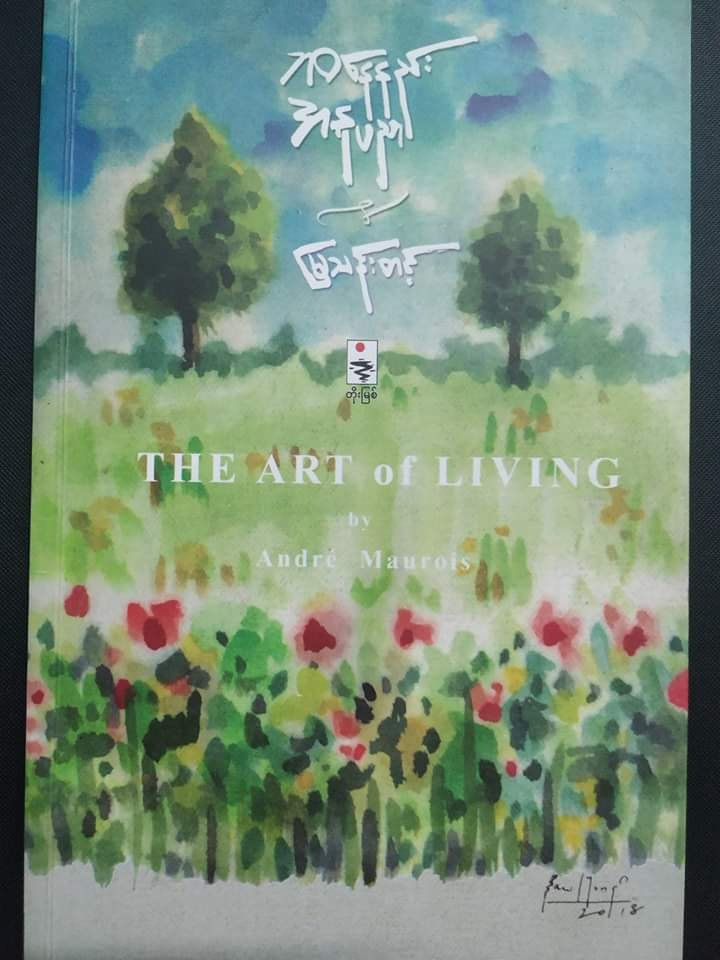
\includegraphics[width=0.3\textwidth]{./fig/fig1.png}}
\noindent{\caption{\padauktext ဘဝနေနည်း အနုပညာ - မြသန်းတင့်}}
\end{figure}

\section{\padauktext မြောက်ဖျားက အလွမ်းရာသီ - စံပယ်ဖြူနု}
\noindent {\padauktext \quotes {မြောက်ဖျားက အလွမ်းရာသီ} တဲ့
ဆရာမစံပယ်ဖြူနုရဲ့ အမျိုးသားစာပေဆုရ ဝတ္ထုလေး ပါ။ ဒီစာအုပ်လေးကို သြဂုတ်လ ၇ရက် ကျောင်းစာပေဟောပြောပွဲ မှာ ဆရာမဂျူး က Recommend ပေးလို့ ဖတ်ဖြစ်ခဲ့တယ် ။ \\
မြန်မာနိုင်ငံမြောက်ပိုင်း ကချင်ပြည်နယ်မှာ ၂၀၁၃ခုနှစ် ပြည်တွင်းစစ် ကြောင့် ပြိုကွဲခဲ့ရတဲ့ မိသားစုဘဝတွေအကြောင်း နောက်ခံထားပြီး အစ်မဖြစ်သူက ညီမလေးကို စစ်ပြေးဒုက္ခသည်စခန်းမှာလိုက်ရှာခဲ့တဲ့ ဇာတ်လမ်းလေး\\
အဒေါ်ဖြစ်သူက နုနယ်တဲ့အဖြူထည်စိတ်လေးကို အရောင်ဆိုးခဲ့ရာမှ အဖေတူအမေကွဲ ညီမလေးအပေါ် မကြင်နာနိုင်ခဲ့သော၊ မုန်းခဲ့သော နွယ် (မေသီနွယ်)\\
(ပတ်ဝန်းကျင် ဆိုတာ ကလေးတစ်ယောက်အပေါ် ဘယ်လောက်ထိ လွှမ်းမိုးနိုင်တယ် ဆိုတဲ အချက်လေး၊ နွယ် တက္ကသိုလ်ရောက်လို့ သိနားလည်လာတာတောင်မှ ငယ်စဉ်ကလေးဘဝက ရိုက်ထည့်ခံခဲ့ရတဲဆူး နှုတ်မရပုံ)\\
ကလေးပီပီ ရိုးသားဖြူစင်လွန်းစွာ အစ်မဖြစ်သူက ကြင်ကြင်နာနာ မရှိသော်လည်း အစ်မအပေါ် တွယ်တာသော အဆိုင်း (မရန်ဆိုင်းမိုင်)\\
အဆိုင်း အိမ်ထောင်ကျပြီး နောက် နေထိုင်ရာ ကချင်ရွာလေးမှာ စစ်ပြေးသွားခဲ့ပြီဆိုတဲ့ သတင်းကလွဲ ဘာမှမသိရတဲ့အခါ ဖခင်ဖြစ်သူက စုံစမ်းပေးဖို့ တောင်းဆိုရာက နွယ့် ရဲ့ မသိစိတ်ထဲက ညီမလေးအပေါ် ချစ်တဲ့စိတ် ၊ စိုးရိမ်စိတ်တွေ ပွင့်ထွက်လာကာ ညီမကို ရှာပုံတော်ဖွင့်ပုံ \\
အဆိုင်းကို ရှာဖွေတဲ့ ခရီးစဉ်မှာ ပါကထောင်၊ အင်ခေါင်းပါ၊ ခါးခယ် စတဲ့ စစ်ပြေးဒုက္ခသည်စခန်းတွေကို ခက်ခက်ခဲခဲ သွားရပုံ \\
တဆက်တည်းမှာပဲ စစ်ပြေးဒုက္ခသည်တို့ရဲ့ ဒုက္ခအဖုံဖုံနဲ့ နေထိုင်စားသောက်ရပုံ \\
ညီမလေး အဆိုင်း ကို ရှာတွေ့ပေမယ့် စာဖတ်သူတွေ မမျှော်လင့်ထားတဲ့ဇာတ်သိမ်းမျိုး နဲ့ \\}
\quotes {\padauktext ကျွန်မတော့ လင်းထင်လောက်မပြောတတ်ပါဘူး။ ဒါပေမဲ့ စစ်ကိုတော့ မုန်းတာအမှန်ပဲ၊ ရှင်ကွဲ သေကွဲ ကွဲကြရမှာ မသေဘဲကျန်ခဲ့ရင်တောင် စိတ်ဒဏ်ရာကျန်ခဲ့မှာကိုတွေးမိတိုင်းမုန်းတယ်။ သမိုင်းမှာဘယ်တုန်းကမှ မကောင်းခဲ့ပေမယ့် ကမ္ဘာမှာ ခုထိစစ်က ပျောက်မသွားဘူးပဲ၊ စစ်ဆိုတဲ့စကားလုံး သိပ်မုန်းတာပဲ၊ ခုပိုတောင်မုန်းလာသေးတယ်}}\\
\noindent {\padauktext
မိုးရာသီသည် ကချင်မြေအဖို့\\
ကံမကောင်းခြင်းကိုသာ\\
လက်ဆောင်လိုယူလာခဲ့ပါသည်ဆိုလျှင်\\
ဆောင်းရာသီကတေ့ာ သူ့အတွက်အိပ်မက်ဆိုးများသာ\\
ပေးခဲ့ပါသည်ဟု အဆိုင်း ဆိုချင်ပါသည်။\\
ဘဝတွင် ယောင်၍မျှ မစဉ်းစားဖူးသော\\
အိပ်မက်ဆိုးပင်တည်း။\\
ထိုနှစ်က ဆောင်းရာသီသည်\\
ပုံမှန်လိုပင် ဆိုက်ရောက်လာခဲ့သည်။\\
နှင်းမြူဝေဆိုင်းခြင်းသည်လည်း ပုံမှန်လို။\\
ကြမ်းရှအေးစိမ့်သောလေများ အိမ်ငယ်လေးများထဲသို့\\
တိုးဝှေ့တိုက်ခတ်သည်မှာလည်း ပုံမှန်လို။\\
အရာရာပုံမှန်လို။\\
သို့သော် ပုံမှန်မဟုတ်ဟု ဆိုစရာရှိသည်များကိုလည်း\\
ကြုံလာရပေသည်။\\
စစ်သည် ခြောက်သယောင်းထသည့်တော၌\\
လောင်အပ်သောမီးနှယ် တစ်စစကျယ်ပြန့်လာပြီ။\\}

\begin{figure}[h!]
\centering{
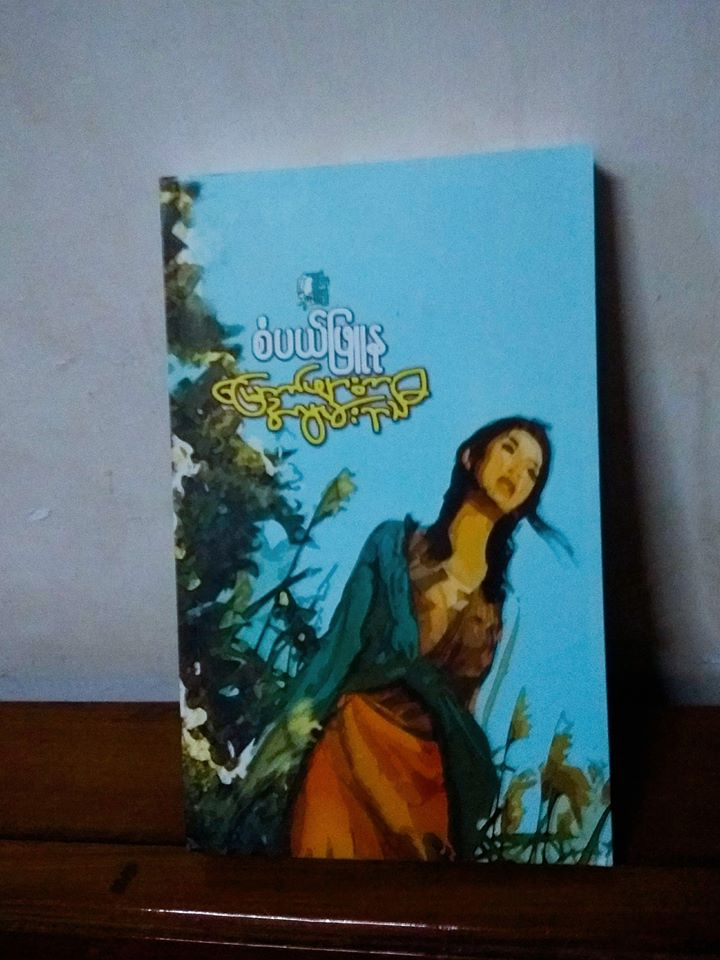
\includegraphics[width=0.3\textwidth]{./fig/fig2.png}}
\noindent{\caption{\padauktext မြောက်ဖျားကအလွမ်းရာသီ - စံပယ်ဖြူနု}}
\end{figure}

\section{\padauktext မေတ္တာရှင်မလေး ပေါ်လီယာနာ - ထင်လင်း}
\noindent {\padauktext \quotes {ဝမ်းသာစရာအကြောင်းကို ရှာတတ်လျှင် ဝမ်းသာစရာအကျိုးဖြစ်ပေါ်၏} တဲ့}\\
\noindent {\padauktext အကောင်းမြင်ဝါဒရှိဖို့အတွက် အသိဉာဏ်တွေ အများကြီးပေးခဲ့တဲ့ မေတ္တာရှင်မလေး \quotes{ပေါ်လီယာနာ}}\\
\noindent {\padauktext ပေါ်လီယာနာ ဆိုတာ အသက် ၁၁ နှစ် အရွယ်သာရှိသေးတဲ့ ကလေးမလေးတစ်ယောက်\\
သူမရဲ့ ထူးခြားချက်က  \\
ဘယ်အရာမဆို ခက်ခဲကြမ်းတမ်းပါစေ \\
ဝမ်းသာစရာအချက်တစ်ခုခု မြင်အောင်ရှာပြီး ဝမ်းသာပစ်လိုက်သည် ။ ကျေးဇူးတင်ပစ်လိုက်သည် ။ \\
ပေါ်လီယာနာက ဒါကို \quotes {ဝမ်းသာတမ်းကစားနည်း} တဲ့ \\
သူမရဲ့ အထူးအဆန်း ဝမ်းသာတမ်းကစားနည်း နဲ့ ပတ်ဝန်းကျင်ရှိ သူမနဲ့ ထိတွေ့ဆက်ဆံရသူများသည် နှလုံးမသာ မျက်နှာမလှ ဖြစ်နေရာက ပြုံးတပျော်ပျော် ဖြစ်လာကြသည် ။ \\}
ဒီစာအုပ်ကို ဖတ် ပြီး သွားမြင်တဲ့ အရာက တော့ လူတော်တော်များများ က ကိုယ်မရသေးတဲ့ အရာတွေ ကိုယ်မပိုင်ဆိုင်ဖြစ်သေးတဲ့ အရာ တွေကိုသာ မျှော်လင့်တောင့်တရင်းနဲ့ ကိုယ်ပိုင်ဆိုင်ထားပြီးသား လက်ရှိအရာတွေအပေါ် ဝမ်းသာကျေနပ်ရမှာ မေ့နေတတ်ကြပါတယ် ။ အောက်စဖို့ဒ် ဆရာတော် ဟောထားသလို လူတွေဟာ မိမိ ပိုင်ဆိုင်ထားတဲ့ အရာတွေ အပေါ်မှာလည်း မုဒိတာ ပွား ဝမ်းမြောက်ရမယ် တဲ့ ။ ကျွန်မ မှာ ခြေနှစ်ဖက် လက်နှစ်ဖက် အင်္ဂါအစုံအလင် ပါလာလို့ ဝမ်းမြောက်တယ် ။ ကျွန်မ မှာ ကျန်းမာနေတဲ့ မိခင် တစ်ယောက် သက်ရှိရှိနေလို့ ဝမ်းမြောက်တယ် ။ ကျွန်မ မှာ စည်းလုံးချစ်ခင်တဲ့ မိသားစုလေး ရှိနေလို့ ဝမ်းမြောက်တယ် ။ ကျွန်မ ဘွဲ့ရ တဲ့ထိ ပညာကောင်းကောင်းသင်ခဲ့ရလို့ ဝမ်းမြောက်တယ် ။ ကျွန်မ လုပ်ချင်တာ တွေ လုပ်နေဖို့ ခုချိန်ထိ အသက်ရှင်နေသေးတာကို ဝမ်းမြောက်တယ် ။ စသည် စသည်ဖြင့် မိမိ မှာ ပိုင်ဆိုင်ထားသော အရာတွေအပါ်မှာ ဝမ်းမြောက်စရာ ၊ မိမိ မပိုင်ဆိုင်လိုသော အရာများ ရှိမနေတဲ့အတွက် ဝမ်းမြောက်စရာ ။\\
ကရုဏာ မုဒိတာ မေတ္တာများနဲ့ ရှင်သန်နေထိုင်ကြစေဖို့ စိတ်ဓာတ်ခွန်အားပေးမဲ့ ပေါ်လီယာနာ ကို မဖတ်ဖူးလျှင် ဖတ်ကြည့်စေချင်စေပါသည်။ \\
ကျွန်မချစ်သော ပေါ်လီယာနာ သည် လူတိုင်း၏ နှလုံးသားတွင် စီးဆင်းနိုင်ကာ လူအများသည်လည်း ဝမ်းသာတမ်း ကစားနည်း အတိုင်း ဝမ်းသာတတ်ကြပါစေ ၊ မေတ္တာထားနိုင်ကြပါစေ ဟု ...}

\begin{figure}[h!]
\centering{
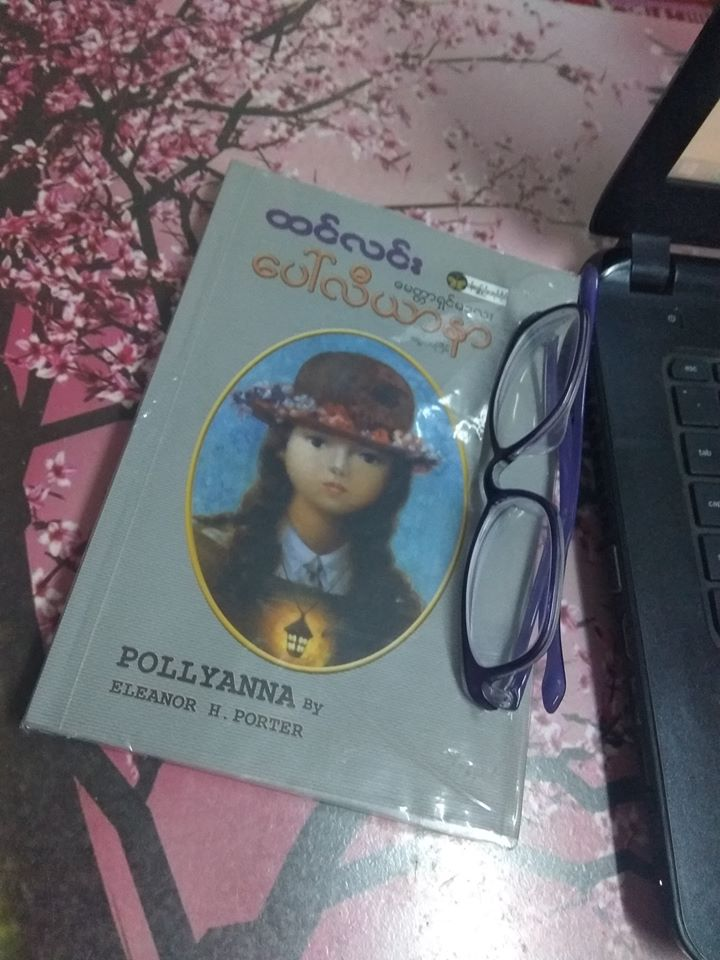
\includegraphics[width=0.3\textwidth]{./fig/fig3.png}}
\noindent{\caption{\padauktext မေတ္တာရှင်မလေး ပေါ်လီယာနာ - ထင်လင်း}}
\end{figure}
\begin{table}[h!]
\caption{\label{table:other recommended books} My Favorite other books}
\noindent{\padauktext အထက်ဖော်ပြပါ စာအုပ် သုံးအုပ် အပြင် ကျွန်မ ဖတ်ဖူးတဲ့အထဲ မှာ အခြားနှစ်သက်မိတဲ့ စာအုပ်တွေကို လည်း list လုပ်ပေးလိုက်ပါတယ်။}
\begin{center}
\begin{tabular}{ |c|c|c| } 
 \hline
 \bf No. & \bf Title & \bf Author \\ [5pt]
 \hline
 1  & \padauktext {ငြိမ်းကိုရှက်ပါ} & \padauktext {မိုးမိုး(အင်းလျား)}\\[5pt]
 \hline
 2  & \padauktext {တက်စ်} & \padauktext {မောင်ထွန်းသူ}\\[5pt]
 \hline
 3  & \padauktext {မြေစာပင်} & \padauktext {ကိုစိုးထိုက်(ဖဒို)}\\[5pt]
 \hline
 4 & \padauktext {အလွမ်းဆိုင်} & \padauktext {စံပယ်ဖြူနု}\\[5pt]
 \hline
 5 & \padauktext {သွေး} & \padauktext {ဂျာနယ်ကျော်မမလေး}\\[5pt]
 \hline
 6 & \padauktext {မာလာရီ} & \padauktext {ဂျာနယ်ကျော်မမလေး}\\[5pt]
 \hline
 7 & \padauktext {ရေနံ့သာခင်ခင်ကြီး} & \padauktext {မောင်သိန်းဆိုင်}\\[5pt]
 \hline
\end{tabular}
\end{center}
\end{table}

\section{Conclusion}
\label{sec:conclusion}
{\padauktext လူငယ်လူရွယ်များ အတွက် စာပေသည် အရေးကြီးသော အခန်းကဏ္ဍတစ်ရပ် အဖြစ် မည်ကဲ့သို့ ပါဝင်နေကြောင်း နှင့် ကျွန်မ ဖတ်ဖူးသမျှထဲ မှာ အကောင်းဆုံး ဖြစ်မည် ဟု ယူဆ ထားသော စာအုပ် သုံးအုပ် အကြောင်းကိုလည်း ဖော်ပြထား ပါသည် ။ မြန်မာပြည် တစ်နံတစ်လျား ရှိ လူငယ်မောင်မယ် တို့ "စာပေ လေ့လာ ဖတ်ရှုမှတ်သား" နိုင် ကြပါစေသည်း။}

\section*{Acknowledgment}

I would like to thank Dr. Ye Kyaw Thu for his homework about "recommended books" with Latex. Thank you so much for the opportunity to learn about Latex especially for Myanmar Language. Thank to Dr. Hnin Aye Thant for the opportunity to attend NLP Class of Software Lab., UTYCC, Pyin Oo Lwin, Myanmar.

\end{document}
